\chapter{Análisis de señales en base a coeficientes respecto a las BLDs}
\label{chap: Analisis de señales en base a coeficientes respecto a las BLDs}
Fijada una dimensión $n$, 
en este capítulo vamos a explicar cómo la 
la base de Legendre discreta $\cali{L}^{n}$ definida en 
\ref{def: base de Legendre discreta}
es una BON que cumple satisfactoriamente los dos puntos de
la lista de deseos
\ref{lista de objetivos}
(que es la motivación de todo este trabajo).



Adicionalmente, en la sección 
\ref{Relación entre proyecciones a espacios de polinomios discretos y aproximaciones por mínimos cuadrados}
estudiamos la estrecha relación que existe entre
proyecciones a los espacios $W_{n,i}$ y a aproximaciones
polinomiales por mínimos cuadrados.


\section{Expresiones de señales finitas respecto a BLDs}

\marginnote{Aquí verificamos que la base de Legendre discreta $\cali{L}^{n}$ 
de $\IR^{n}$ satisface el primer punto de la lista de deseos 
\ref{lista de objetivos}.}

Puesto que por definición se realizó un proceso de ortonormalización
para obtener a $\cali{L}^{n}$, este primer punto se cumple trivialmente.

\begin{obs}
Sean $n \geq 2$, $\cali{L}^{n}$ la BLD definida en 
\ref{def: base de Legendre discreta}.
Para toda $x \in \IR^{n}$ se tiene que 
\[
x = \suma{k=0}{n-1}{\left\langle x, \cali{L}^{n,k} \right\rangle 
\cali{L}^{n,k}}
\]
y
\[
|| x ||^{2} = \suma{k=0}{n-1}{\left\langle x, \cali{L}^{n,k} \right\rangle^{2}}.
\]
\end{obs}

\noindent A la luz del teorema de la proyección ortogonal, 
las proyecciones de $x$ sobre los espacios 
$W_{n,0}$, $W_{n,1}$
y $W_{n,2}$ son los vectores
de estos espacios más cercanos (en términos de la 
distancia euclídea)
a $x$; es natural entonces formular
las siguientes definiciones.

\marginnote{Puede recordar la definición
de proyección ortogonal, basada en la unicidad
establecida en el 
teorema de la proyección ortogonal \label{Teo:proyOrt},
en \eqref{eq3: 1Dic}.}


\begin{defi}
Si $x \in \IR^{n}$ y
\begin{equation}
\label{eq0: 5Dic}
\Pi_{W_{n,i}}: \IR ^{n}  \longrightarrow W_{i}, \hspace{0.2cm}
i=0,1,2
\end{equation}
son las proyecciones ortogonales
a los espacios 
$W_{n,0}$, $W_{n,1}$ y $W_{n,2}$, a los vectores
\[
\Pi_{W_{n,i}}(x), \hspace{0.2cm} i=0,1,2
\]
les llamaremos la \textbf{parte constante}
o \textbf{promedio}, la \textbf{parte afín} y la
\textbf{parte cuadrática}, respectivamente, de $x$.
\end{defi}

\begin{prop}
\label{prop: proyecciones a espacios Wn,k}
Sea $x \in \IR^{n}$; si
\[
x= \suma{k=0}{n-1}{\left\langle x, \cali{L}^{n,k} \right\rangle\cali{L}^{n,k}},
\]
entonces, para toda $0 \leq i \leq n-1$,
\[
\Pi_{W_{n,i}}(x)=\suma{k=0}{i}{\left\langle x, \cali{L}^{n,k} \right\rangle\cali{L}^{n,k}}
\]
y
\[
||\Pi_{W_{n,i}}(x)||^{2}=\suma{k=0}{i}{\left\langle x, \cali{L}^{n,k} \right\rangle^{2}}
\]
\end{prop}
\textbf{Demostración.}
Sólo recuerde que, para toda $0 \leq i \leq n-1$,
los vectores $\cali{L}^{n, j}$ con $0 \leq j \leq i$
conforman una BON de $W_{n,i}$
(c.f. corolario \ref{cor: BON de legendre para espacios Wk}) y
que $a_{k}= \langle x, \cali{L}^{n,j} \rangle$.
Use el corolario \ref{cor: proyeccion en terminos de una BON}.
\QEDB 
\vspace{0.2cm}

\begin{ejemplo}
\label{subs: ejm 2}

Considere al siguiente conjunto de cinco
puntos del plano:
\begin{equation} \label{eq: conjunto cinco puntos}
\{ (0,-0.5), (1,2.4), (2, 1.6), (3,1.7), (4, 2.3) \}.
\end{equation}
Como tenemos cinco puntos, trabajamos
en el espacio $\IR^{5}$. 

El vector cuyas entradas
son las cinco mediciones (dadas por las ordenadas
de los puntos del conjunto \eqref{eq: conjunto cinco puntos})
es
\begin{equation}
\label{eq0: 29Nov}
x=(-0.5, 2.4, 1.6, 1.7, 2.3).
\end{equation}


\begin{figure}[H]
	\sidecaption{
	Gráfica de la señal $x \in \IR^{5}$.
	\label{fig: grafica semal x ejemplo}
	}
	\centering
	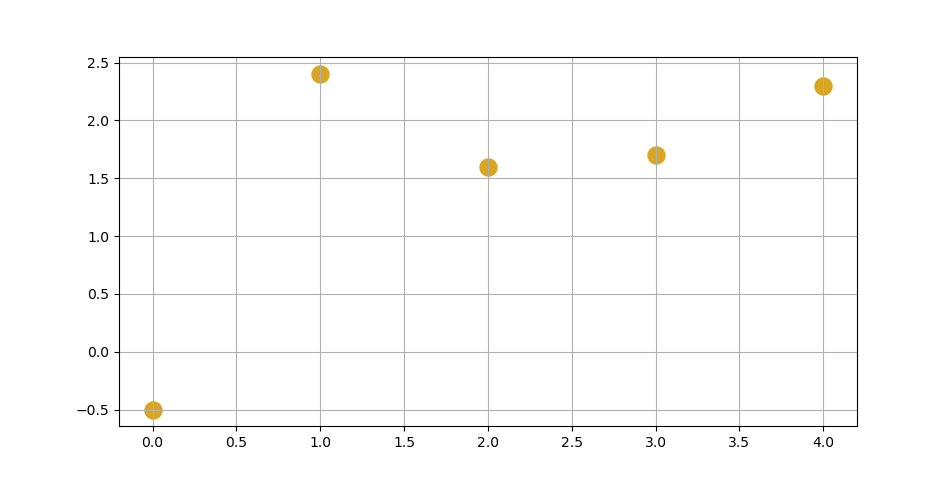
\includegraphics[scale=0.4]{graficaX_31Oct} 
\end{figure}	


Nos interesa
dar explícitamente a 
la señal $\Pi_{W_{5,1}}(x) \in W_{5,1} \leq \IR^{5}$.
En realidad, por ser $\cali{L}^{5}$ 
una base ortonormal de $\IR^{5}$ y por ser
$W_{5,1}$ el subespacio generado por los
dos primeros vectores de esta base, 
se sabe de inmediato que
\[
\Pi_{W_{5,1}}(x)=  \langle \Pi_{W_{5,1}}(x), \cali{L}^{5,0} \rangle \cali{L}^{5,0}
+ \langle \Pi_{W_{5,1}}(x), \cali{L}^{5,1} \rangle \cali{L}^{5,1};
\]
de todas formas, como ilustración, planteemos un sistema
de ecuaciones para llegar a una expresión para
$\Pi_{W_{5,1}}(x)$.
Usando las expresiones para los vectores
de $\cali{L}^{5}$
dadas en \ref{subsect:Formulas explicitas},
tenemos que
\[
W_{5,1}=span\{ (1,1,1,1,1,1), (-2, -1, 0, 1, 2) \},
\]

y 
\[
W_{5,1}^{\perp}=span\{ (2,-1,-2,-1,2), (-1,2,0,-2,1), (1,-4,6,-4,1)\}.
\]
Según el teorema de la proyección ortogonal \ref{Teo:proyOrt},
$\Pi_{W_{5,1}}(x)$ es el único elemento de $W_{5,1}$ para el 
que 

\[
x-\Pi_{W_{5,1}}(x) \in W_{5,1}^{\perp};
\]
esto se 
traduce en la existencia de 
únicos escalares $c_{1}$, $c_{2}$,
$a_{1}$, $a_{2}$ y $a_{3}$ tales que
\[
x-c_{1}(1,1,1,1,1)-c_{2}(-2, -1, 0, 1, 2)
\]
es igual a 

\[
a_{1}(2,-1,-2,-1,2)+a_{2}(-1,2,0,-2,1)
+ a_{3}(1,-4,6,-4,1),
\]
\noindent
o sea, tales que

\begin{equation*}
\begin{cases}
-0.5-(c_{1}-2c_{2})=2a_{1}-a_{2}+a_{3}, \\
2.4-(c_{1}-c_{2})=-a_{1}+2a_{2}-4a_{3}, \\
1.6-c_{1}=-2a_{1}+6a_{3},\\
1.7-(c_{1}+c_{2})=-a_{1}-2a_{2}-4a_{3}, \\
2.3-(c_{1}+2c_{2})=2a_{1}+a_{2}+a_{3}.
\end{cases}
\end{equation*}
Resolviendo este sistema
de ecuaciones, encontramos que
$c_{1}=1.5$ y $c_{2}=0.49$. Así,




\begin{align}
\label{eq0: 8ab}
\Pi_{W_{5,1}}(x) =& c_{1} (1,1,1,1,1) + c_{2}(-2-1,0,1,2) \nonumber \\
= & (0.52, 1.01, 1.5, 1.99, 2.48 );
\end{align}

observe que 
la regresión lineal calculada a partir
del conjunto de datos
\eqref{eq: conjunto cinco puntos}
es la recta
con ecuación cartesiana

\begin{equation} \label{eq: recta minimos cuadrados}
y=0.49x+0.52
\end{equation}

y que \eqref{eq0: 8ab} es, 
como se asegura en la proposición
\ref{prop: discretizacion recta minimos cuadrados}, la discretización de 
la recta \eqref{eq: recta minimos cuadrados}
en la malla uniforme $\cali{P}_{5}$.
De forma análoga se calcula la parte cuadrática de
la señal $s$.

\begin{figure}[H]
	\sidecaption{
	Gráficas de $x$, 
	$\Pi_{W_{5,0}}(x)$, $\Pi_{W_{5,1}}(x)$ y $\Pi_{W_{5,2}}(x)$.
	\label{fig: partes afin, lineal y cuadratica} 
	}
	\centering
	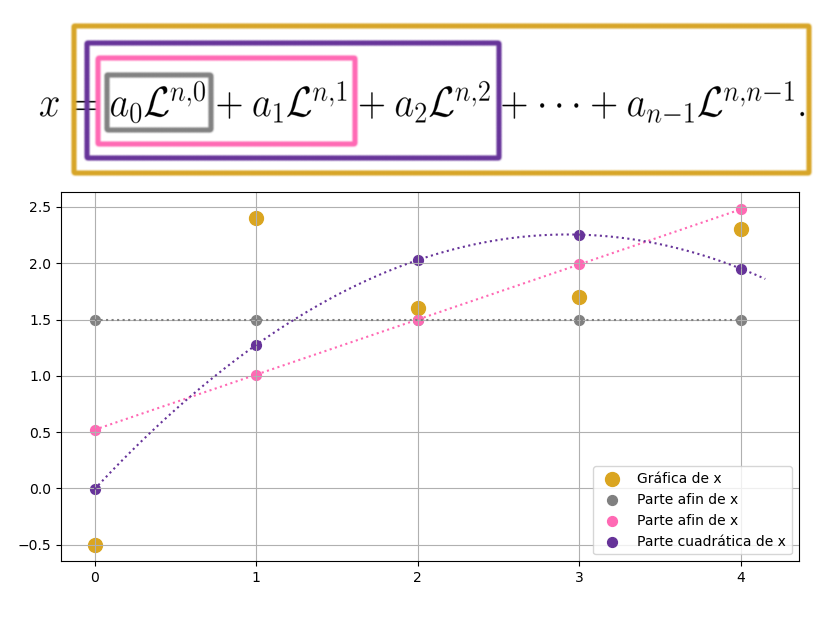
\includegraphics[scale=0.6]{parteAfinCuadr}
\end{figure}	
\final
%Final ejemplo 2--------------------------------------------
\end{ejemplo}


\section{Caracterización de morfología en base a coeficientes respecto a las BLDs}
\label{Caracterización de la morfología en términos de coeficientes respecto a la base de Legendre discreta}

\marginnote{Aquí verificamos que la base de Legendre discreta $\cali{L}^{n}$ 
de $\IR^{n}$ satisface el segundo punto de la lista de deseos 
\ref{lista de objetivos}.}

Ahora que contamos con bases ortonormales
para los espacios de polinomios discretos
(c.f. corolario \ref{cor: BON de legendre para espacios Wk}),
es sencillo reescribir al corolario
\ref{Teorema1},
en el que se dan condiciones necesarias y suficientes para que
una señal sea afín o cuadrática,
no en términos de pertenencia a espacios de polinomios
discretos,
sino en términos de coeficientes.


\begin{prop} 
\label{prop: condiciones necesarias y suficientes sobre la forma de x en terminos de los espacios Wi}
Sean $n \in \IN$, $\cali{L}^{n}$
la base de Legendre discreta de dimensión $n$
definida en 
\ref{def: base de Legendre discreta} y
$x \in \IR^{n}$ una señal de dimensión $n$. 

\noindent
Se tiene que la señal $x$ es
 
\begin{itemize}
\item constante si y sólo si para todo índice
$1 \leq k \leq n-1$ se cumple que $\left\langle x, \cali{L}^{n,k} \right\rangle=0$,

\item afín si y sólo si sólo sus primeros
para todo índice
$2 \leq k \leq n-1$ se cumple que $\left\langle x, \cali{L}^{n,k} \right\rangle=0$,

\item cuadrática si y sólo si 
para todo índice
$3 \leq k \leq n-1$ se cumple que $\left\langle x, \cali{L}^{n,k} \right\rangle=0$,
y además $\left\langle x, \cali{L}^{n,k} \right\rangle \neq 0$.
\end{itemize} 

\end{prop}
\noindent
\textbf{Demostración.}
Por ejemplo, para probar el segundo punto, sólo observe que
$x$ es lineal sí y sólo si $x \in W_{n,1}$
(c.f. \ref{cor: condiciones necesarias y suficientes para que x sea afín en términos de pertenencia a espacios Wi}), 
lo que equivale a que $x$ coincida con su proyección
al espacio $W_{n,1}$ que, según la proposición
\ref{prop: proyecciones a espacios Wn,k}
es $\langle x, \cali{L}^{n,0} \rangle \cali{L}^{n,0} + 
\langle x, \cali{L}^{n,1} \rangle \cali{L}^{n,1}$; esta igualdad 
implica que los coeficientes $\langle x, \cali{L}^{n,k} \rangle$
con $k >1$ sean cero. \QEDB
\vspace{0.2cm}




Más aún; a pesar de que
una señal $x$ no sea ni lineal ni cuadrática, gracias a la 
ortogonalidad de la base
$\cali{L}^{n}$ podemos formalizar lo que
entendemos por que una señal se asemeje a ser
afín o cuadrática y, además, \textbf{cuantificar} esta semejanza;
dada una señal $x \in \IR^{n}$ y
su representación respecto a la BON $\cali{L}^{n}$,
como se explica en la observación 
\ref{prop: condiciones necesarias y suficientes sobre la forma de x en terminos de los espacios Wi}, tenemos condiciones necesarias y suficientes
(muy sencillas de comprobar)
\textbf{en términos de los coeficientes $\langle x , \cali{L}^{n,k} \rangle$}
de $x$ respecto a $\cali{L}^{n}$ 
en referencia a la \textbf{forma
de la gráfica de $x$}, pero, incluso aunque no se satisfagan
estas condiciones,
puesto que contamos con la identidad de Parseval
(c.f. nota \ref{nota: sobre la identidad de parseval}),
si
algunos coeficientes $\langle x , \cali{L}^{n,k} \rangle$ son considerados pequeños, estos
pueden eliminarse y obtener así una señal cercana (en distancia
euclídea) a la original que tenga una forma determinada.
Por ejemplo, si todos los coeficientes de una 
$x \in \IR^{n}$ respecto a $\cali{L}^{n}$, a excepción de 
$\langle x , \cali{L}^{n,0} \rangle$,
$\langle x , \cali{L}^{n,1} \rangle$ y
$\langle x , \cali{L}^{n,2} \rangle$,
son pequeños, entonces, a pesar de que
$x$ no pertenezca a $W_{n,2}$ (o sea, no sea cuadrática),
será cercana a ser cuadrática.

\begin{ejemplo}
\label{subs: ejm 3}

En este ejemplo 
damos dos propuestas naturales,
usando los espacios de polinomios discretos $W_{n,k}$,
para poder dar no sólo respuestas del tipo
``sí/no'' a preguntas sobre la morfología de una señal, sino,
de forma más general, del tipo ``qué tanto sí'' o
``qué tanto no''.



%Inicio ejemplo 3--------------------------------------------

Sea $x \in \IR^{n}$. Digamos que 
\[
x = \suma{k=0}{n-1}{a_{k} \cali{L}^{n, k}}.
\]


Como se argumentó ya, las proposiciones
\begin{center}
``$x \in \IR^{n}$ es afín'' \hspace{0.2cm} y \hspace{0.2cm} 
``$x \in W_{n,1}$''
\end{center} 
son equivalentes.
Observe que, aún cuando no se cumpla el caso
extremos de que $x$ sea elemento 
de $W_{n,1}$ (y, por lo tanto, no podamos aseverar que
$x$ es afín), provistos
de nociones como las de norma y ortogonalidad, es fácil dar 
una propuesta legítima de
\textbf{medidas} de ``qué tan afín'' es la señal $x$,
o, en términos matemáticos, de qué tanto se aleja
$x$ del espacio de señales afines de su correspondiente
espacio ambiente.

Como se explica en la subsección \ref{cosine similarity}, hay
dos formas plausibles de dar medidas de qué tan cerca está
$x$ del plano $W_{n,1}$;

\begin{itemize}
\item[a)] Una forma obvia de proceder es calcular
la distancia de $x$ al espacio $W_{n,1}$, que por definición es 
la norma
del vector 
\[
x - \Pi_{W_{n,1}}(x)= \suma{k=2}{n-1}{a_{k} \cali{L}^{n, k}},
\]
es decir, tomar al número no negativo
\[
\sqrt{ \suma{k=2}{n-1}{a_{k}^{2}}}
\]
como una medida de qué tanto se aleja $x$ del plano $W_{n,1}$
(o sea, de qué tanto se aleja $x$ de ser afín).

\item[b)] Otro acercamiento podría ser preguntarse por
el ángulo $\alpha \in [0, \frac{\pi}{2}]$ 
que forma el vector $x$ con
$W_{n,1}$, el espacio de señales afines $n-$dimensionales.
\end{itemize}
Veamos por qué la segunda
es la mejor forma de proceder.

Si $x \in \IR^{n}$ es una señal de dimensión $n$ y 
$a \in \IR-\{ 0 \}$ es un escalar cualquiera,
la gráfica de $a \cdot x$ no es más que la gráfica 
de $x$ reescalada por un factor de $a$ cuando este
último es positivo; en caso contrario, es la gráfica
de $x$ reescalada pero además reflejada respecto al eje
horizontal.

La morfología de la gráfica de $x$ es entonces,
salvo reflexiones horizontales, invariante bajo multiplicación
escalar; otro atributo de $x$ que no se ve afectado por esta acción
es el ángulo que forma con el plano $W_{n,1}$ de señales afines
(c.f. proposición \ref{prop: angulo se conserva bajo mult. esc.}), 
aunque la distancia euclidea de la señal
al plano $W_{n,1}$ por lo general sí es afectada por multiplicaciones escalares.


\begin{figure}[H]
	\sidecaption{ Para $n=3$,
	se grafica a $x$ junto con algunos múltiplos escalares de $x$.
	Observe que, salvo reflexiones horizontales, la gráfica de estas
	señales tiene la misma forma.
	\label{fig: aaa} 
	}
	\centering
	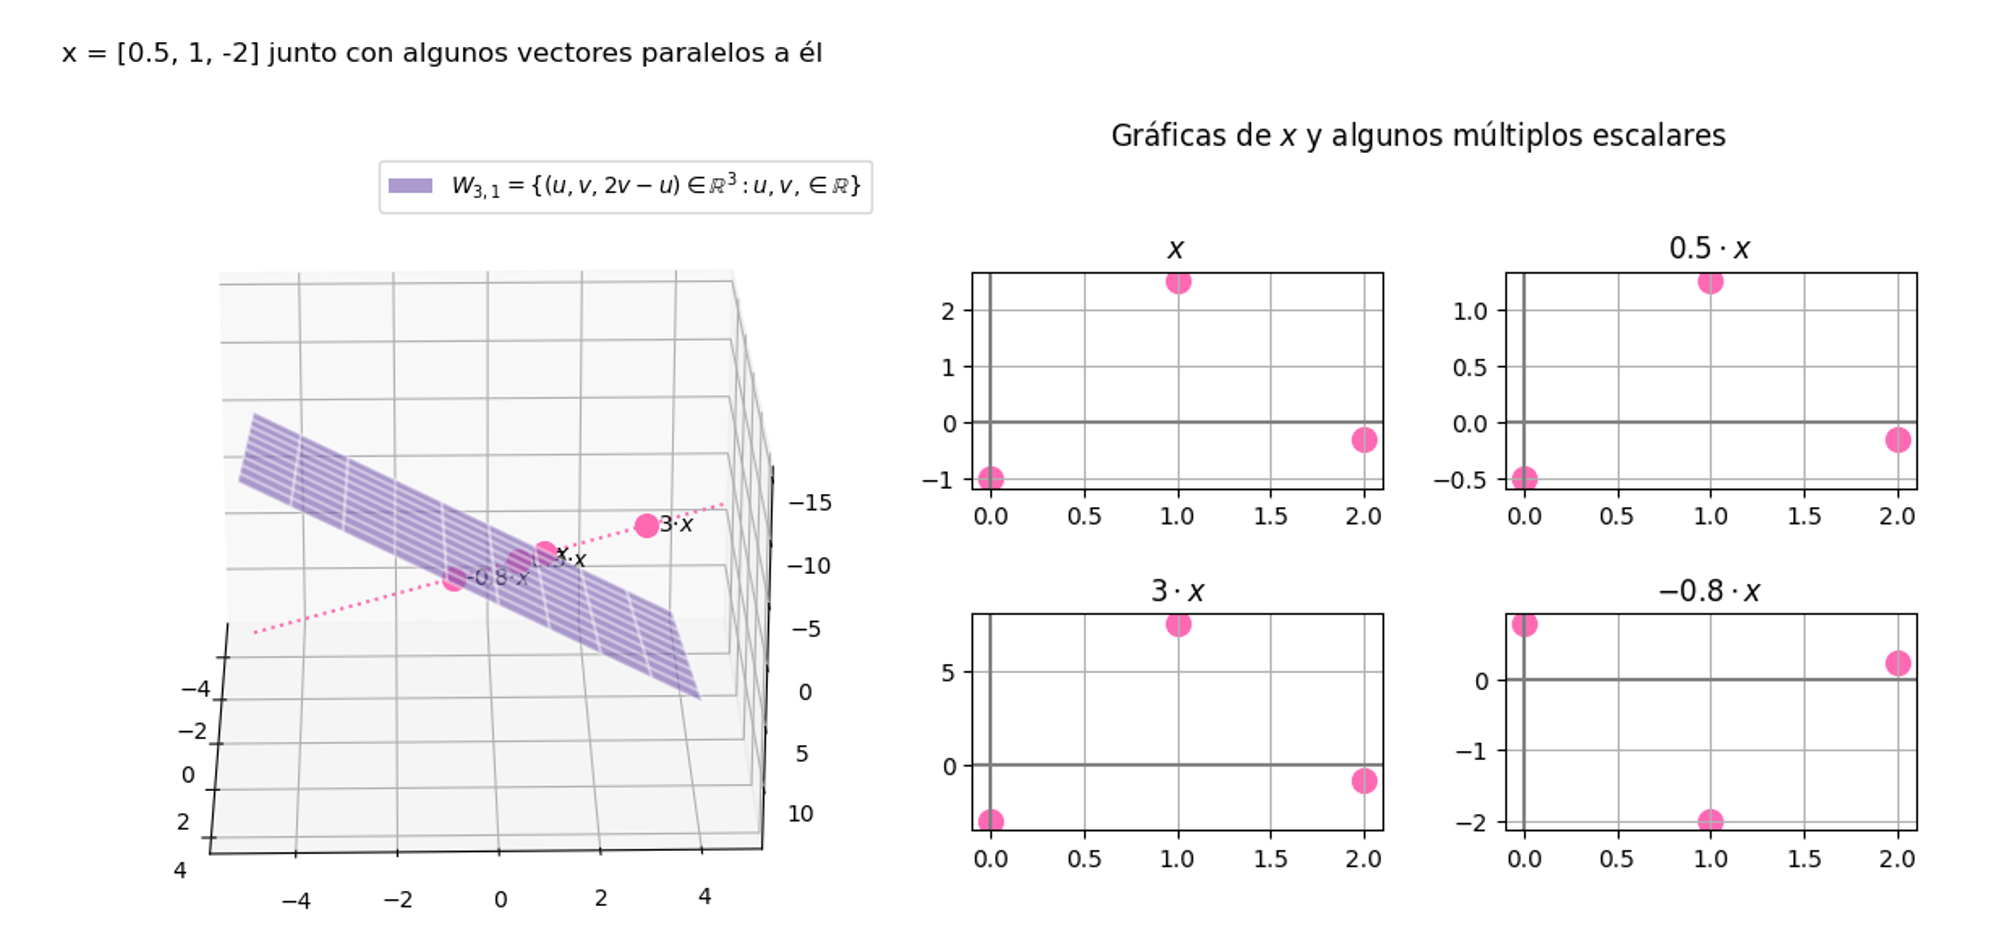
\includegraphics[scale=0.18]{borrador}
\end{figure}

\textbf{Tomamos pues al coseno del ángulo que forma $x$ con su proyección
al plano $W_{n,1}$ como una medida de cercanía de $x$ a la propiedad de 
ser afín.}


Para dar un ejemplo concreto, fijemos $n=3$.
Como se calculó en \eqref{eq2: 1Dic},
el subespacio $W_{3,1} \leq \IR^{3}$ de señales afines es el plano
de ecuación cartesiana

\[
W_{3,1}: \hspace{0.2cm} x-2y+z=0.
\]
Sea 
\begin{equation*}
\label{eq0: 9Feb}
x=a_{0}\cali{L}^{3,0}+a_{1}\cali{L}^{3,1}+a_{2}\cali{L}^{3,2}
\end{equation*}
un vector del espacio.


Como las dimensiones de $\IR^{3}$ y $W_{3,1}$ 
difieren por uno,
este útimo es un hiperplano
\sidenote{Puede recordar la definición
de hiperplano en 
\ref{section: hiperplanos}.}
del primero; como $\cali{L}^{3,2}$
es un vector normal a $W_{3,1}$
(c.f. corolario \ref{cor: Ln,k ortogonal a todo pol discreto de grado menor a k}), 
si $\varphi: \IR^{3} \longrightarrow \IR$ es la función
definida como
\begin{equation}
\label{eq: funcion phi ejemplo}
\varphi(x)= \langle \cali{L}^{3,2} , x \rangle =a_{2},
\end{equation}



las tres regiones ajenas en las
que $W_{3,1}$ divide al espacio
$\IR^{3}$ son 


\begin{itemize}
\item[I)] $\{ x \in \IR^{3} : \varphi(x)>0 \}$,
región a la que pertenece $\cali{L}^{3,2}$,
\item[II)] $W_{3,1}= Ker(\varphi)$, y 
\item[III)] $\{ x \in \IR^{3} : \varphi(x)<0 \}$,
región a la que pertenece $-\cali{L}^{3,2}$.
\end{itemize}

\begin{figure}[H]
	\sidecaption{Se ilustran las tres 
		regiones en las que $W_{3,1} \subseteq \IR^{3}$ divide al espacio,
		clasificadas según el signo que tome 
		la función $\varphi$ como se definió en
		\eqref{eq: funcion phi ejemplo}. En
		{\color{ameDorado}{dorado}} se muestra al vector
		$\cali{L}^{3,2}$, en {\color{ameRosa}{rosa}}
		un elemento de la región citada, y en 
		{\color{ameMorado}{morado}} la proyección de este
		al espacio $W_{3,1}$.
	\label{fig: angulo x y proy} 
	}
	\centering
	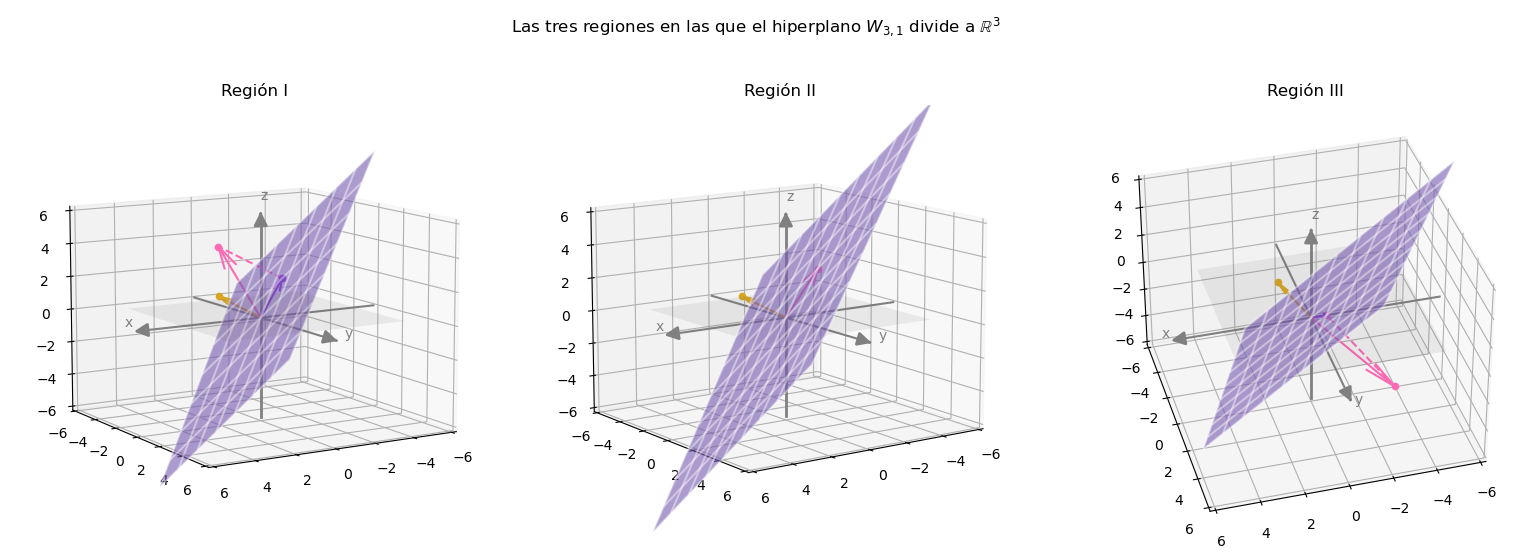
\includegraphics[scale=0.3]{2Dic_4} 
\end{figure}

Es fácil obtener una expresión para el coseno del ángulo
$\alpha$ en términos de los coeficientes de $x$ respecto a $\cali{L}^{3}$:

\begin{figure}[H]
	\sidecaption{Encontrando una fórmula explícita del 
	ángulo que forma $x$ con $\Pi_{W_{3,1}}(x)$.
	\label{fig: angulo x y proy} 
	}
	\centering
	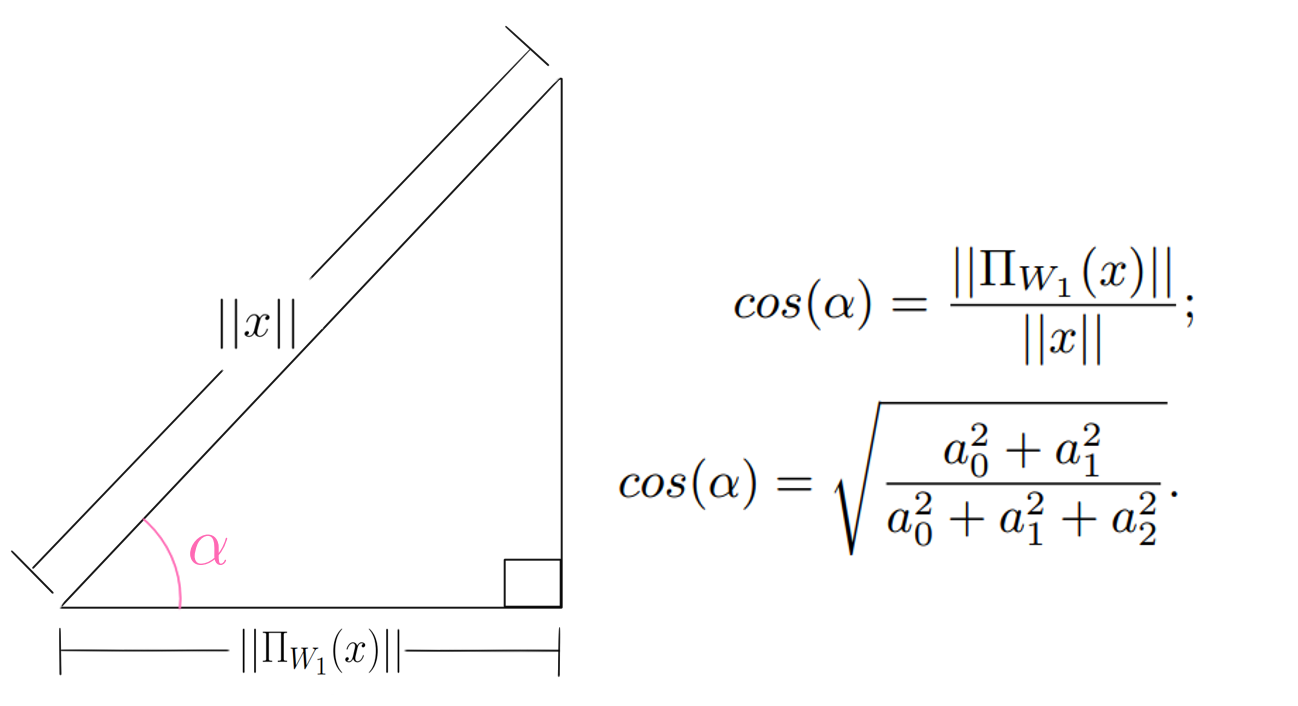
\includegraphics[scale=0.7]{2Dic_3}
\end{figure}


De las relaciones de la figura 
\ref{fig: angulo x y proy} 
obtenemos una igualdad que relaciona el ángulo 
$\alpha$ que forma una señal $x \in \IR^{3}$ 
con su proyección al espacio $W_{3,1}$
con los coeficientes $a_{i}$
de $x$ respecto a $\cali{L}^{3}$:
\begin{equation}
\label{eq0: 3Dic}
cos(\alpha)= \sqrt{\frac{a_{0}^{2}+a_{1}^{2}}{a_{0}^{2}+a_{1}^{2}+a_{2}^{2}}}.
\end{equation}

Para un ejemplo aún más concreto, hagamos 
\begin{equation}
\label{eq1: 19Sept}
a_{0}= \sqrt{3}, \hspace{0.2cm} a_{1}= \sqrt{2},
\end{equation}


\noindent
es decir, consideremos a todos los vectores de $\IR^{3}$
cuya proyección al plano $W_{3,1}$ es 
el vector
\begin{equation}
\label{eq1: 6Dic}
(0,1,2).
\end{equation}
Es obvio que el conjunto de los puntos
del espacio cuya proyección a
$W_{3,1}$ es \eqref{eq1: 6Dic} de hecho la recta
con ecuación vectorial
\begin{equation}
\label{eq0: 6Dic}
l_{(0,1,2)} := (0,1,2)+c(1,-2,1), \hspace{0.2cm} c \in \IR.
\end{equation}

\noindent
Sustituyendo
los valores \eqref{eq1: 19Sept} en \eqref{eq0: 3Dic} y
despejando
\sidenote{
En general, si $C:= || \Pi_{W_{3,1}}(x) || ^{2}$,
entonces $a_{2}^{2}= C \cdot4 tg^{2}(\alpha).$
}, obtenemos 
\[
|a_{2}|= \sqrt{5 tg^{2}(\alpha)};
\]
el signo del coeficiente $a_{2}$ (que corresponde a la dirección
de $\cali{L}^{3,2}$ en la descomposición de $x$) se determina por
la región en la que se encuentre $x$;

\begin{itemize}
\item el signo de $a_{2}$ es positivo si $x$ es elemento de la región I,
\item $a_{2}=0$ si $x$ es elemento de la región II, y
\item el signo de $a_{2}$ es negativo si $x$ es elemento de la región III.
\end{itemize}


Grafiquemos ahora algunos elementos
de la recta \eqref{eq0: 6Dic}.
Los valores de las entradas de $x$, en la
mayoría de los casos, han sido redondeados.


\begin{figure}[H]
	\sidecaption{Aquí se considera al vector 
		$x$ que forma un ángulo $\alpha=\pi/3$
		con el plano $W_{3,1}$ y que se ubica en la región I.
	\label{fig: angulo x y proy} 
	}
	\centering
	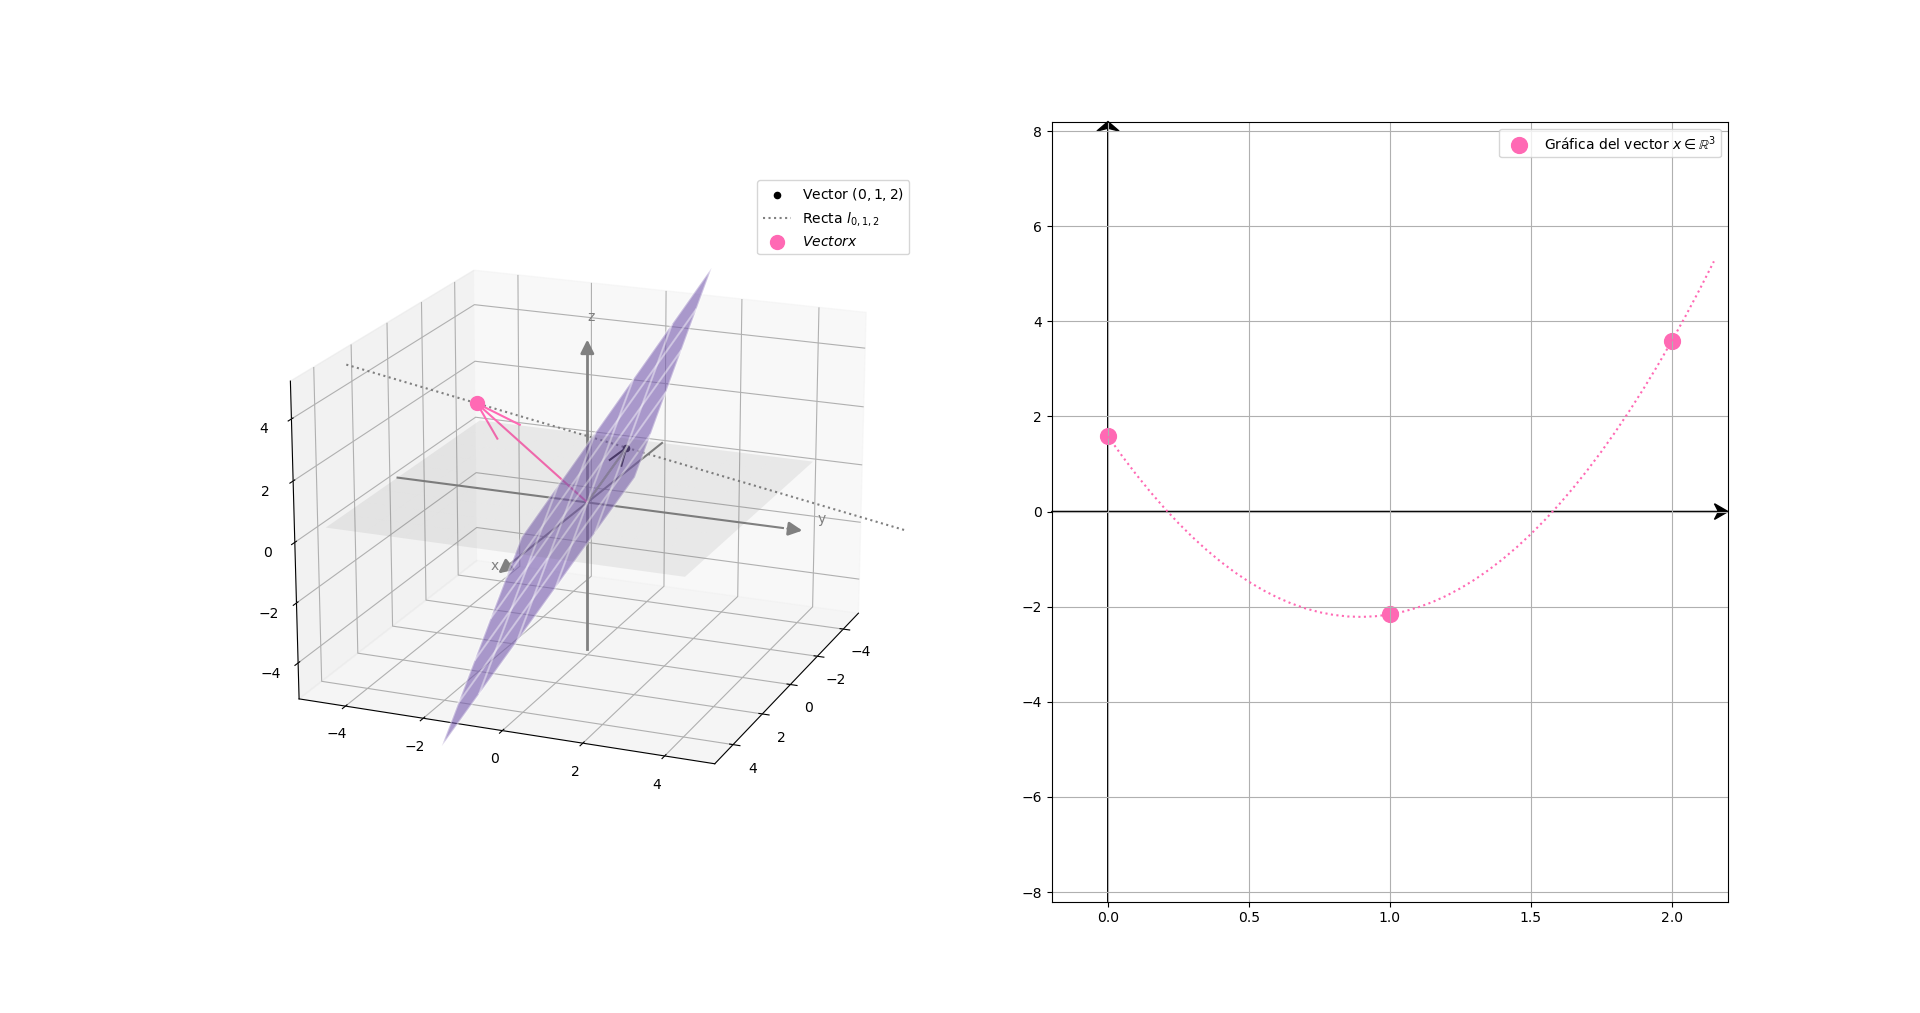
\includegraphics[scale=0.3]{6Dic_0}
\end{figure}



\begin{figure}[H]
	\sidecaption{Aquí se considera al vector 
		$x$ que forma un ángulo $\alpha=\pi/3$
		con el plano $W_{3,1}$ y que se ubica en la región I.
	\label{fig: angulo x y proy} 
	}
	\centering
	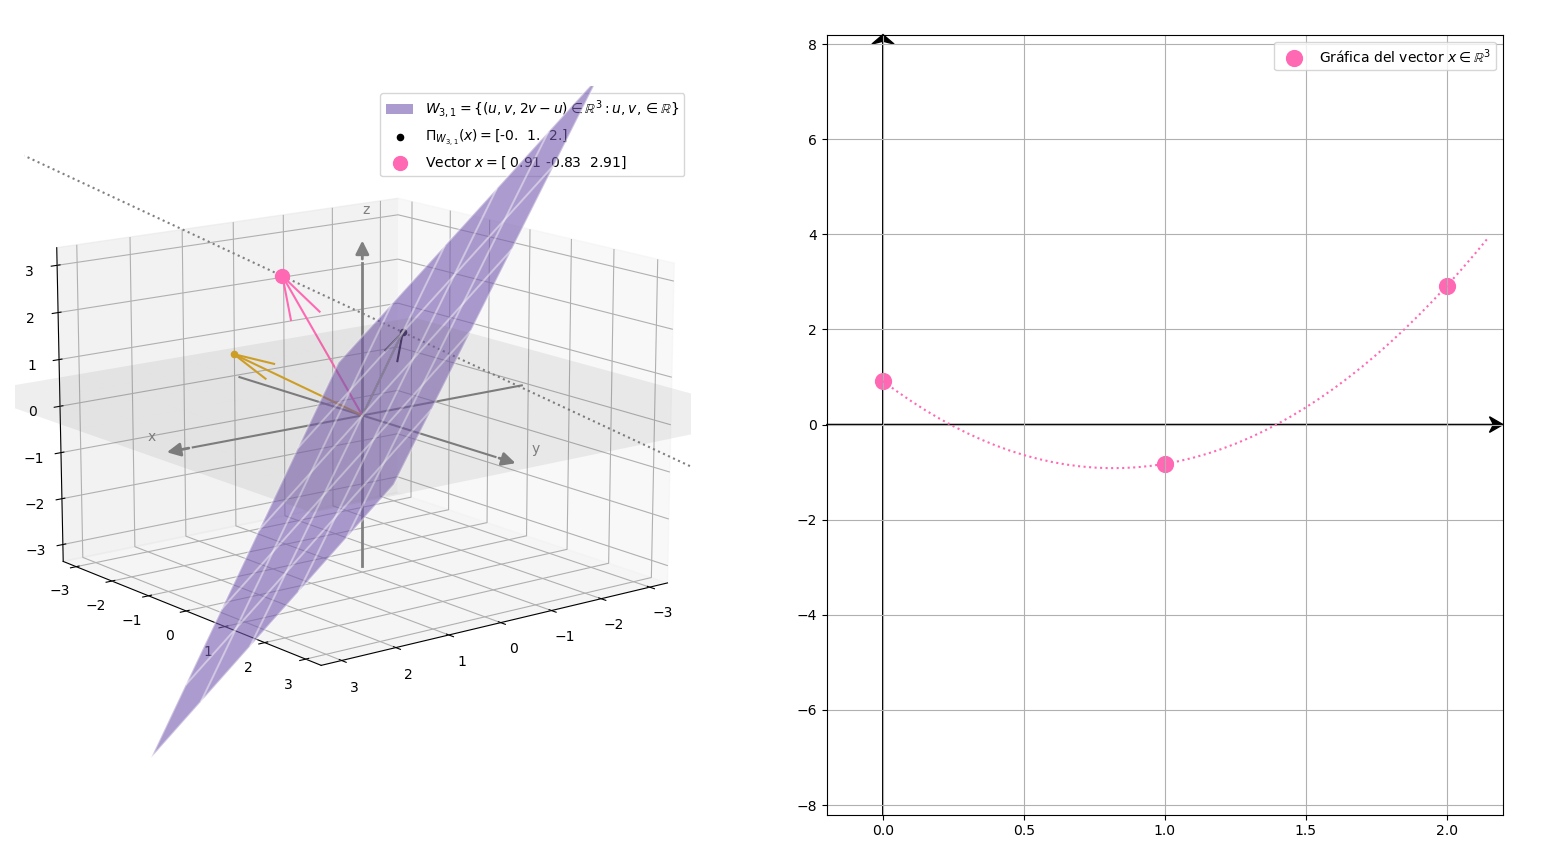
\includegraphics[scale=0.3]{6Dic_1}
\end{figure}

\begin{figure}[H]
	\sidecaption{Aquí se considera al vector 
		$x$ que forma un ángulo $\alpha=0$
		con el plano $W_{3,1}$ y que se ubica en la región II.
	\label{fig: angulo x y proy} 
	}
	\centering
	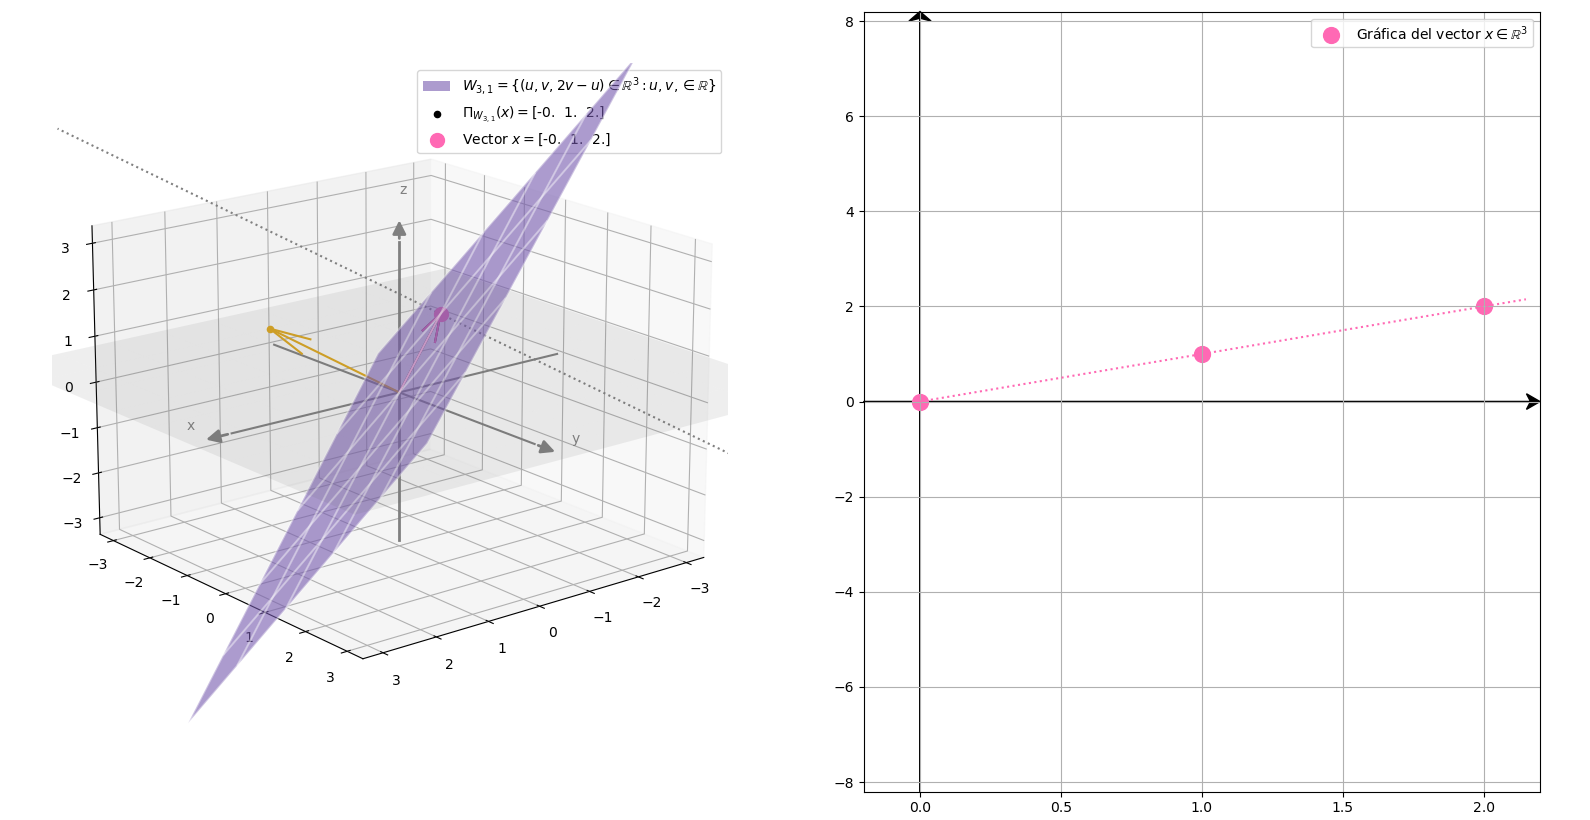
\includegraphics[scale=0.3]{6Dic_2}
\end{figure}

\begin{figure}[H]
	\sidecaption{Aquí se considera al vector 
		$x$ que forma un ángulo $\alpha=\pi/3$
		con el plano $W_{3,1}$ y que se ubica en la región III.
	\label{fig: angulo x y proy} 
	}
	\centering
	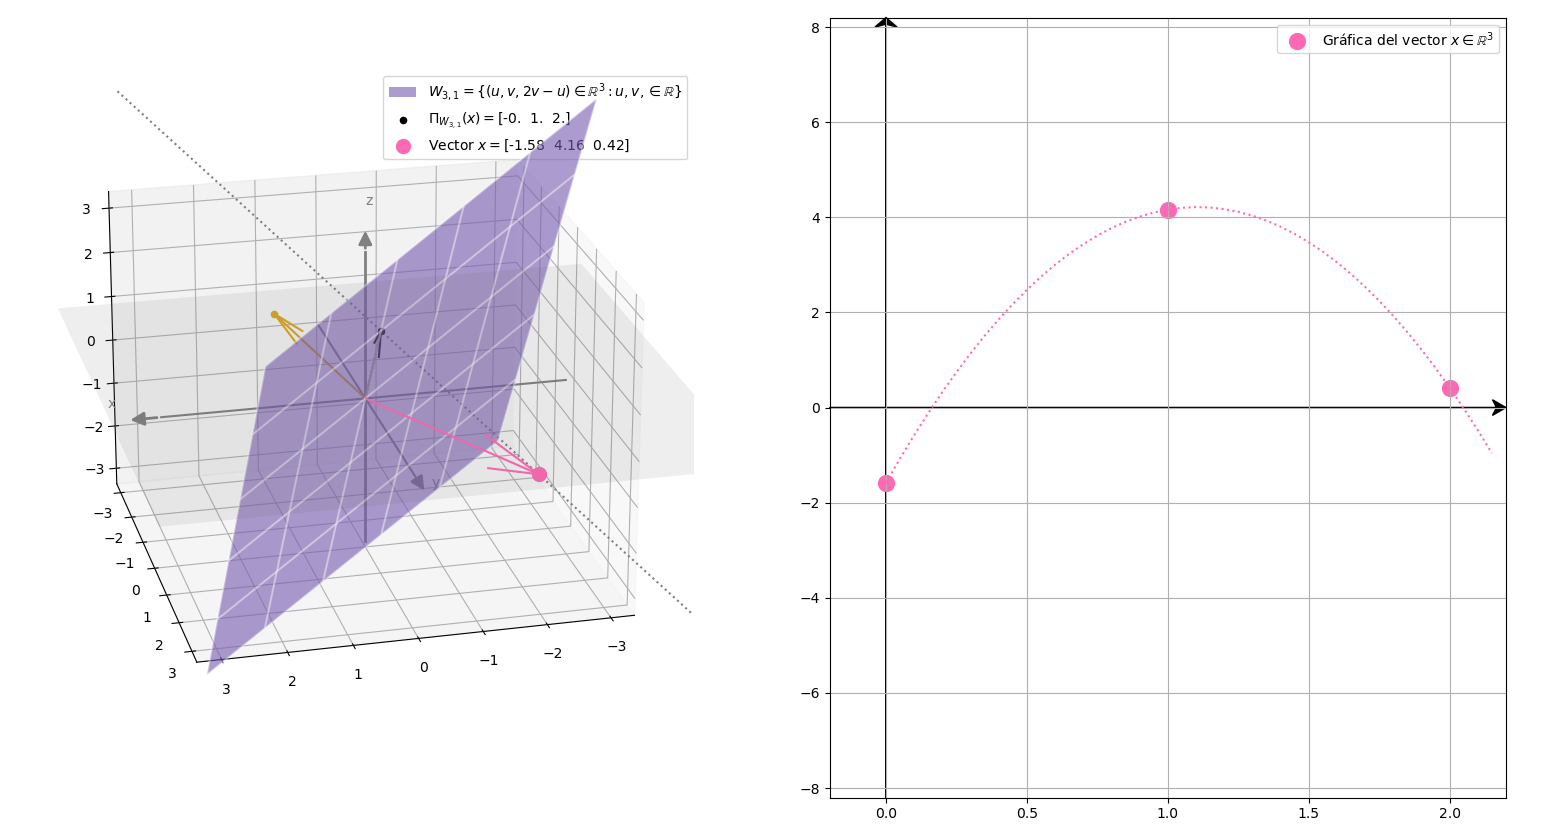
\includegraphics[scale=0.3]{6Dic_3}
\end{figure}

\begin{figure}[H]
	\sidecaption{Aquí se considera al vector 
		$x$ que forma un ángulo $\alpha=6\pi/17$
		con el plano $W_{3,1}$ y que se ubica en la región III.
	\label{fig: angulo x y proy} 
	}
	\centering
	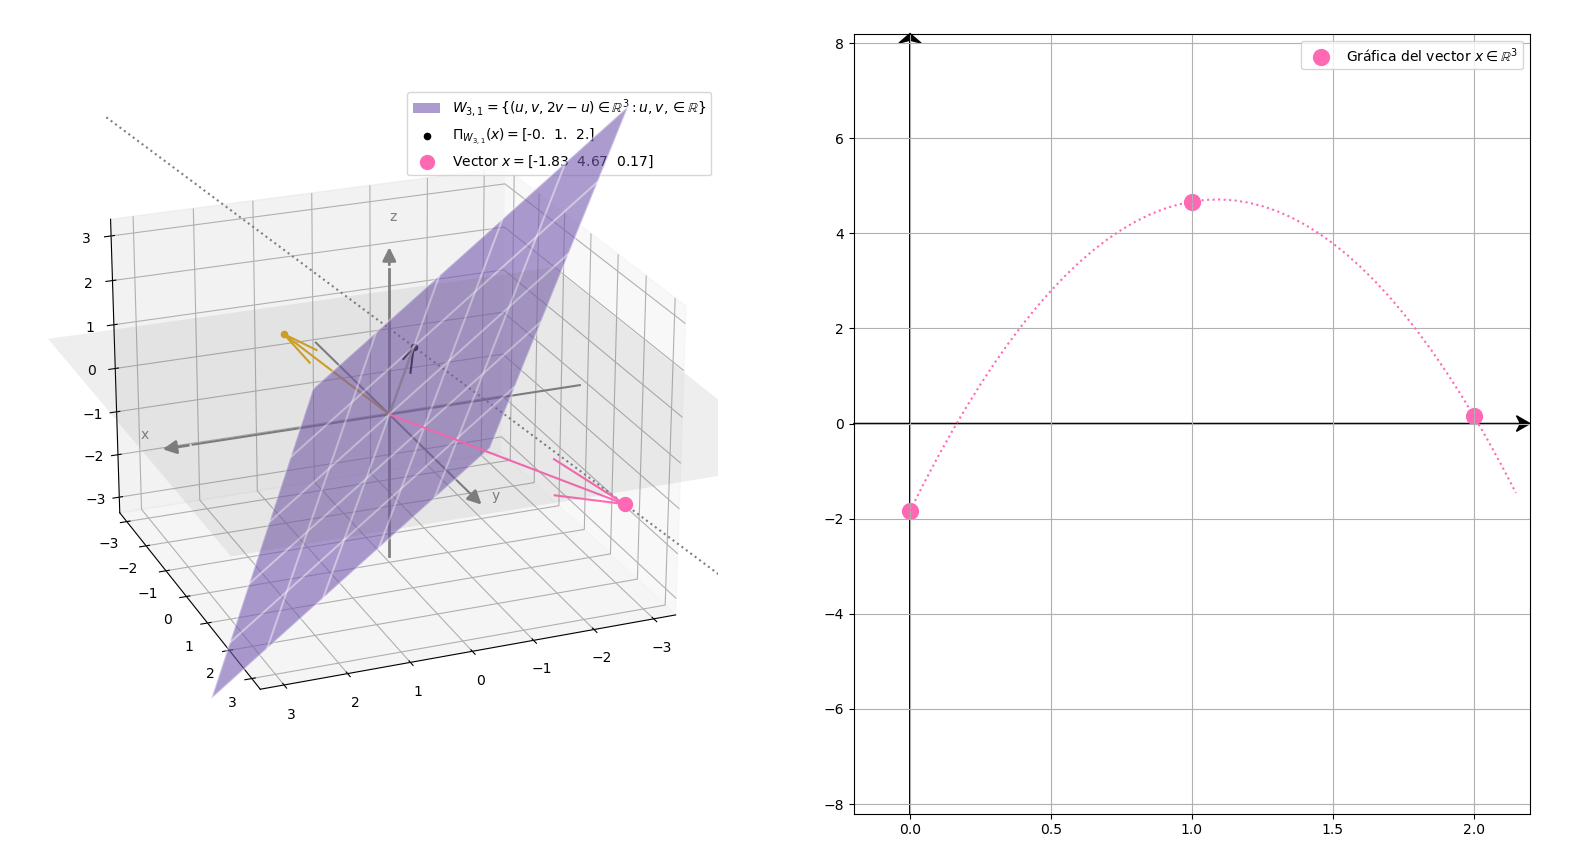
\includegraphics[scale=0.3]{6Dic_4}
\end{figure}


%Final ejemplo 3--------------------------------------------
\final
\end{ejemplo}





%-----------------------------------------------------

\section{Relación entre proyecciones a espacios de polinomios discretos y aproximaciones por mínimos cuadrados}
\label{Relación entre proyecciones a espacios de polinomios discretos y aproximaciones por mínimos cuadrados}

Hasta el momento, hemos partido siempre
de una señal $x \in \IR^{n}$
y, a partir de ella, considerado al subconjunto $G_{x}$ 
de $\IR^{2}$ (interesándonos por patrones de 
recta y parábola que este pueda seguir).
Si, recíprocamente, se tiene un 
subconjunto de puntos de $\IR^{2}$ 
\begin{equation}
\label{eq: Halloween!}
G:=\{(j, x_{j}): 0 \leq j \leq n-1 \},
\end{equation}
con $n \geq 2$,
cuyas abscisas formen una malla uniforme
de $n$ puntos, tenemos ahora dos caminos
para dar una aproximación lineal
que modele el comportamiento 
seguido por estos puntos:

\begin{enumerate}
\item El clásico método de
mínimos cuadrados, método que, en este contexto,
consiste en minimizar a la función
de dos variables 
\begin{equation}
\label{eq: funcion a minimizar}
\mu (m,b)= \suma{j=1}{n}{(x_{j}-(mj+b))^{2}},
\end{equation}
es decir, en encontrar una pendiente
$m_{0} \in \IR$ y un $b_{0} \in \IR$ 
para los que la suma de las distancias
al cuadrado entre las mediciones 
(i.e. los valores $x_{j}$)
y los valores correspondientes de la función
$l_{min}(t):=m_{0}t+b_{0}$
sea mínima. 


\begin{figure}[H]
	\sidecaption{
	Partimos del conjunto $G$
	cuyos elementos son $(0, 5)$,
	$(1, 3.2)$, $(2, 4.6)$, $(3,0)$
	y $(4,-0.3)$, y
	calculamos la
	recta de mínimos cuadrados correspondiente
	a este conjunto, que resulta ser 
	$l_{min}: y =-1.38t+5.26$.
	\label{fig: proyeccion vs minimos cuadrados 1}
	}
	\centering
	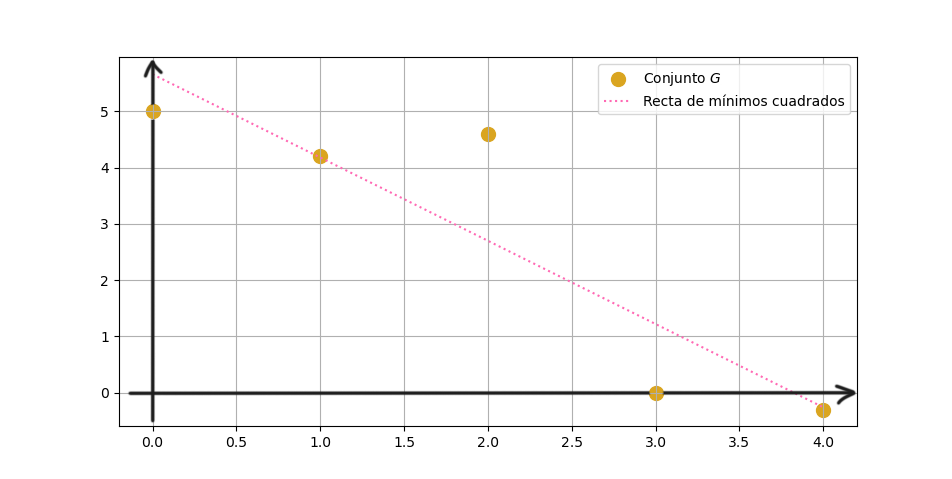
\includegraphics[scale= 0.55]{2Dic_1} 
\end{figure}	


\item Considerar al vector $x=(x_{j})_{j=0}^{n-1}$
de $\IR^{n}$, proyectarlo al espacio $W_{n,1}$ 
de polinomios discretos de dimensión $n$ y grado uno
y usar
a la recta $l_{x}$ cuya discretización en 
$\cali{P}_{n}$ sea esta proyección
$\Pi_{W_{n,1}}(x) \in W_{n,1}$ 
(que existe por ser precisamente
$W_{n,1}$ el espacio de discretizaciones
de polinomios discretos de dimensión $n$ con
grado a lo más uno, c.f. 
teorema \ref{cor: propiedades importantes de espacios Wi})
como aproximación lineal del conjunto \eqref{eq: Halloween!}.


\begin{figure}[H]
	\sidecaption{	
		El vector formado a partir
		del conjunto $G$ 
		de la figura 
		\ref{fig: proyeccion vs minimos cuadrados 1}
		es $x=(5,3.2,4.6,0,-0.3)$.
		Su proyección al espacio $W_{5,1}$ es
		$\Pi_{W_{5,1}}(x)= (5.26, 3.88,
		2.5, 1.12, -0.26)$, y la recta
		cuya discretización en $\cali{P}_{5}$	
		es la señal $\Pi_{W_{5,1}}(x)$ es
		$l_{x}: y=-1.38t+5.26$.
	\label{fig: proyeccion vs minimos cuadrados 2}
	}
	\centering
	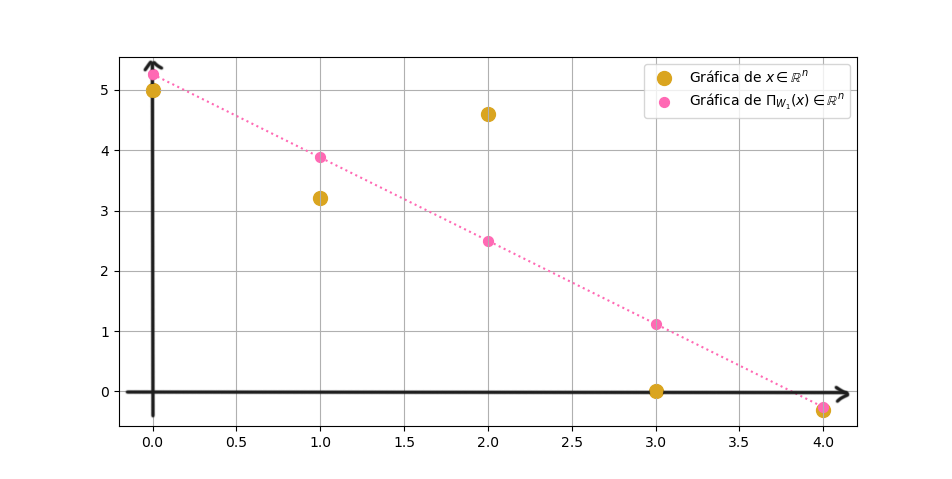
\includegraphics[scale= 0.55]{2Dic_2} 
\end{figure}	

\end{enumerate}


Puesto que el mínimo 
$(m_{0}, b_{0})$ de la función 
\eqref{eq: funcion a minimizar} siempre existe,
y como siempre puede formarse el vector
$x=(x_{j})_{j=0}^{n-1}$ a partir del conjunto $G$
dado en \eqref{eq: Halloween!} 
y proyectarse este
a $W_{n,1}$, los dos caminos discutidos arriba
son siempre realizables.


\noindent Como establecemos en la siguiente observación, estas
dos formas de abordar el problema de aproximación
coinciden. Observe que la demostración de este hecho 
no es más que una consecuencia directa del 
teorema de la proyección \ref{Teo:proyOrt}
pues, hablando en los términos que hemos
usado hasta ahora, encontrar la recta de mínimos
cuadrados de la 
gráfica $G_{x}$ es lo mismo que encontrar al elemento
del espacio $W_{n,1}$ cuya distancia euclidea a $x \in \IR^{n}$
sea mínima.


\begin{prop}
\label{prop: discretizacion recta minimos cuadrados}
Sea $n \geq 2$ y sea el conjunto de $n$ puntos del plano
\begin{equation}
\label{eq10: 10Dic}
\{(j, x_{j}): 0 \leq j \leq n-1 \}
\subseteq \IR^{2}.
\end{equation}
Si $x=(x_{j})_{j=0}^{n-1}$ es la señal cuya
gráfica $G_{x}$ coincide con el conjunto dado
en \eqref{eq10: 10Dic}, si
\begin{itemize}
\item $l_{min}: y= m_{0}t+ b_{0}$ es la recta obtenida 
aproximando los puntos del conjunto \eqref{eq10: 10Dic}
con el método de mínimos cuadrados, y

\item $l_{x}$ es la recta cuya versión discreta 
respecto a la malla uniforme $\cali{P}_{n}$
es $\Pi_{W_{n,1}}(x) \in \IR^{n}$, 

\end{itemize} 
entonces las rectas $l_{x}$ y $l_{min}$ coinciden.
\end{prop}
\noindent 
\textbf{Demostración.}
Si demostramos que las señales
\[
r:= \Omega_{n, \cali{P}_{n}}(l_{min}) \in \IR^{n}
\]
y
\[
\Pi_{W_{n,1}}(x) \in W_{n,1} \subseteq \IR^{n}
\]
coinciden, podremos concluir la 
igualdad entre las rectas $l_{x}$ y $l_{min}$
(pues la igualdad $r= \Pi_{W_{n,1}}(x)$
significa que las rectas $l_{min}$ y $l_{x}$
{coinciden en los puntos con abscisas los elementos
de $\cali{P}_{n}$, que son al menos dos).

Por ser $r$ la discretización
en una malla uniforme de un
polinomio de grado uno, es elemento del espacio $W_{n,1}$
(c.f. teorema 
\ref{cor: propiedades importantes de espacios Wi}). 
Además, si $z$ es cualquier señal afín
(es decir, cualquier elemento de $W_{n,1}$)
y si $y=mt+b$
es la ecuación de la recta sobre la que yace su gráfica,
por definición de $l_{min}$ sabemos que

\begin{equation}
\label{eq0: 5Enero}
\suma{j=1}{n}{(x_{j}-(m_{0}j+b_{0}))^{2}}
=\mu(m_{0}, b_{0}) \leq \mu(m, b)= 
\suma{j=1}{n}{(x_{j}-(mj+b))^{2}};
\end{equation}
\noindent 
tomando raíces cuadradas 
en ambos extremos de \eqref{eq0: 5Enero}
llegamos a la desigualdad
\[
d(x, r) \leq d (x,z)
\]
(donde $d$ denota a la distancia euclidea en $\IR^{n}$).
Como $z$ fue un elemento arbitrario del espacio $W_{n,1}$,
inferimos que

\[
d(x, r)  = \text{inf} \{ d (x,z) : z \in W_{n,1} \};
\]
de la unicidad establecida en el teorema de la proyección
ortogonal \ref{Teo:proyOrt} concluimos que $r= \Pi_{W_{n,1}}(x)$. \QEDB
\vspace{0.2cm}


Aquí sólo se trató el caso lineal, pero,
naturalmente, discusiones
totalmente análogas se valen para grados más altos
(estando los grados posibles acotados superiormente
por la cardinalidad del conjunto de puntos $G$
dado en \eqref{eq: Halloween!} 
a aproximar), por 
ejemplo, cuando se buscan
aproximaciones cuadráticas
(resp. cúbicas) para cuando
la cardinalidad del conjunto 
\eqref{eq: Halloween!} es mayor o igual a tres 
(resp. cuatro).